\documentclass[11pt]{beamer}
\usetheme{Ilmenau}
%\usecolortheme{beaver}
%\beamertemplatenavigationsymbolsempty
\usepackage{multimedia}
\usepackage[utf8]{inputenc}
\usepackage{amsmath}
\usepackage{amsfonts}
\usepackage{amssymb}
\usepackage{graphicx}
%\author{}
\title{PP Gruppe 8}
%\setbeamercovered{transparent} 
%\setbeamertemplate{navigation symbols}{} 
%\logo{} 
%\institute{} 
%\date{} 
%\subject{} 
\begin{document}

\frame[c]{\titlepage}
\begin{frame}
\tableofcontents
\end{frame}


\section{Frequenzfilter}
\begin{frame}
	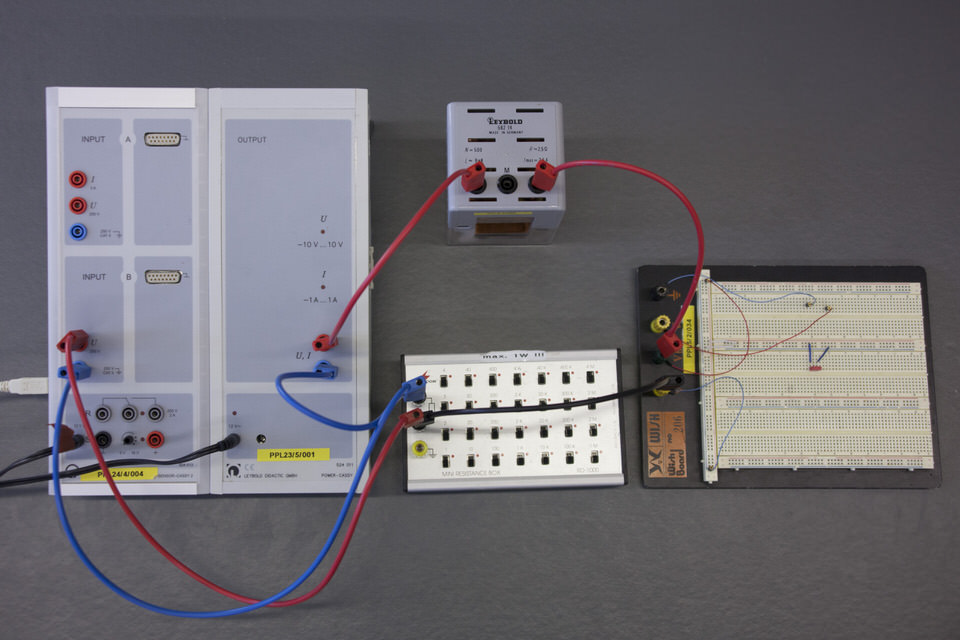
\includegraphics[width=\textwidth]{images/1/durchlassfilter}
\end{frame}

\begin{frame}
	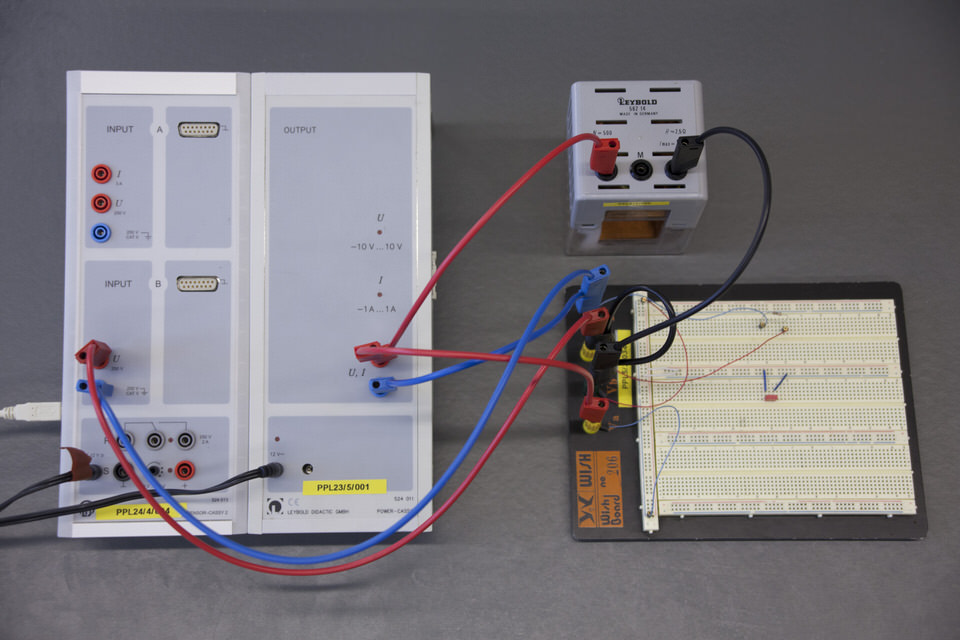
\includegraphics[width=\textwidth]{images/1/sperrfilter}
\end{frame}

\begin{frame}
	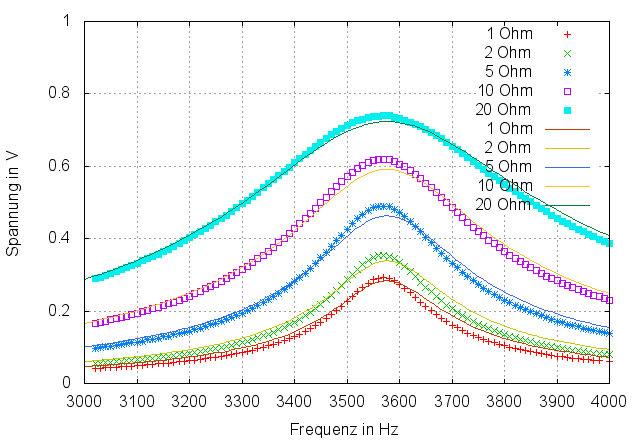
\includegraphics[width=\textwidth]{images/1/plot}
\end{frame}


\section{Michelson-Interferometer}
\begin{frame}
	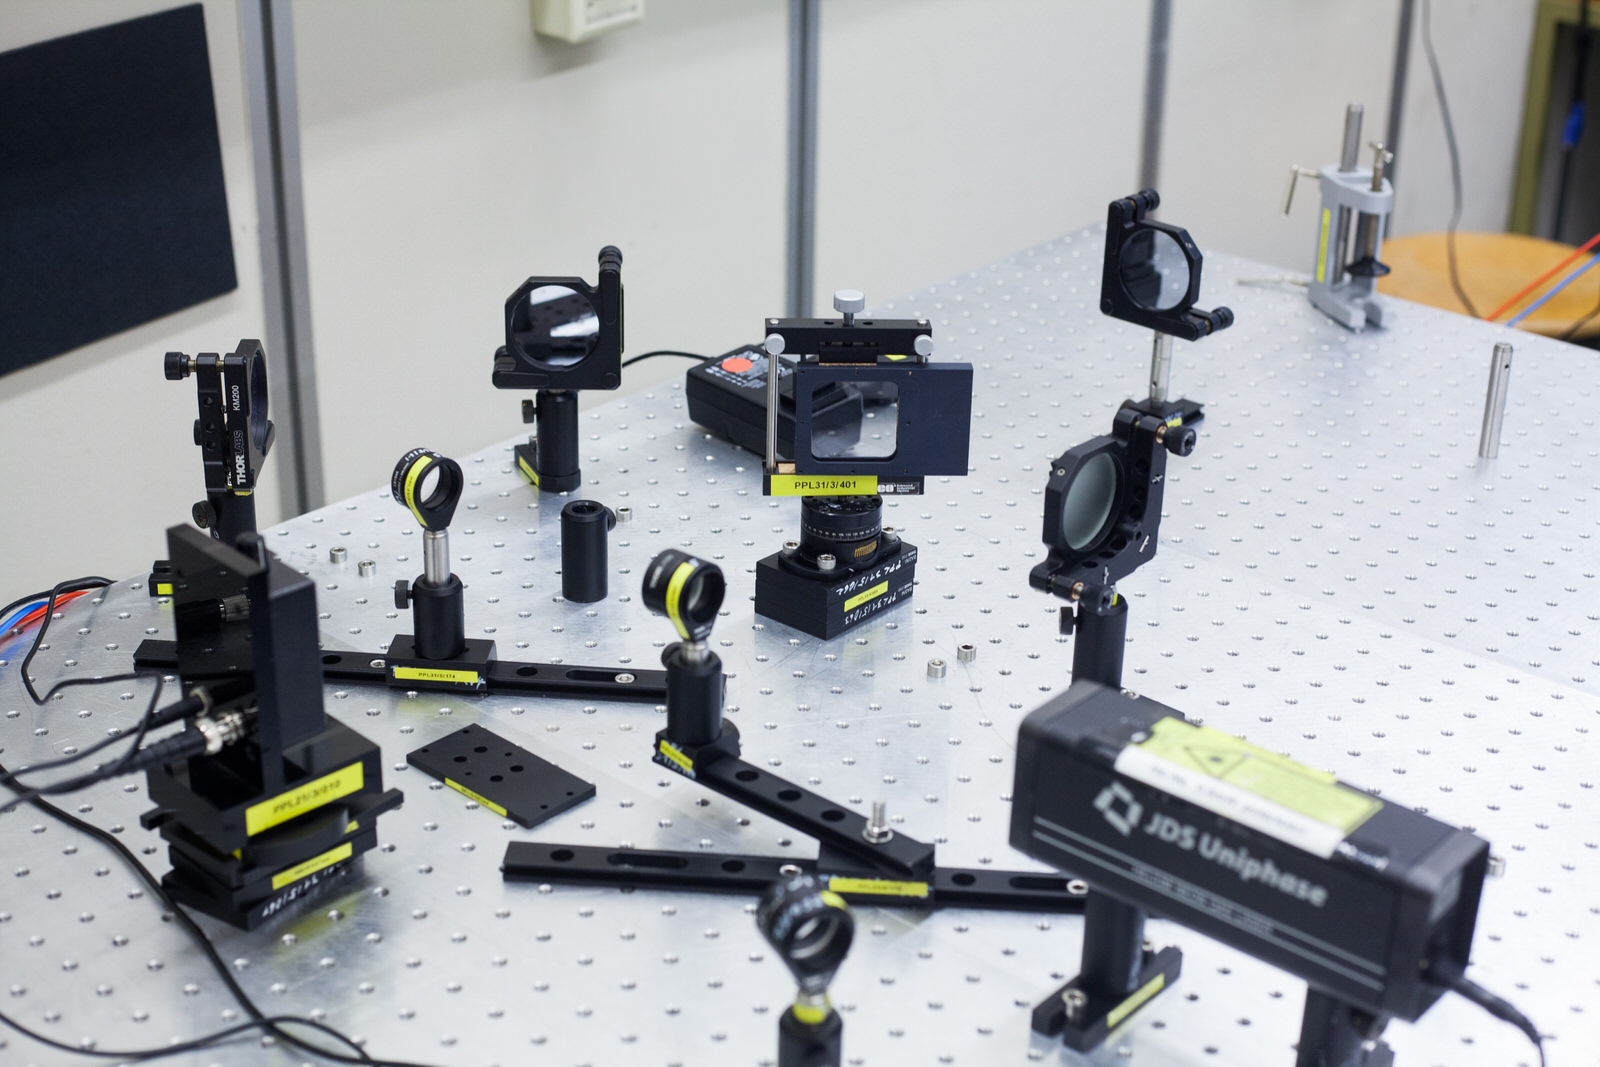
\includegraphics[width=\textwidth]{images/2/interferrometer-4}
\end{frame}

\begin{frame}
	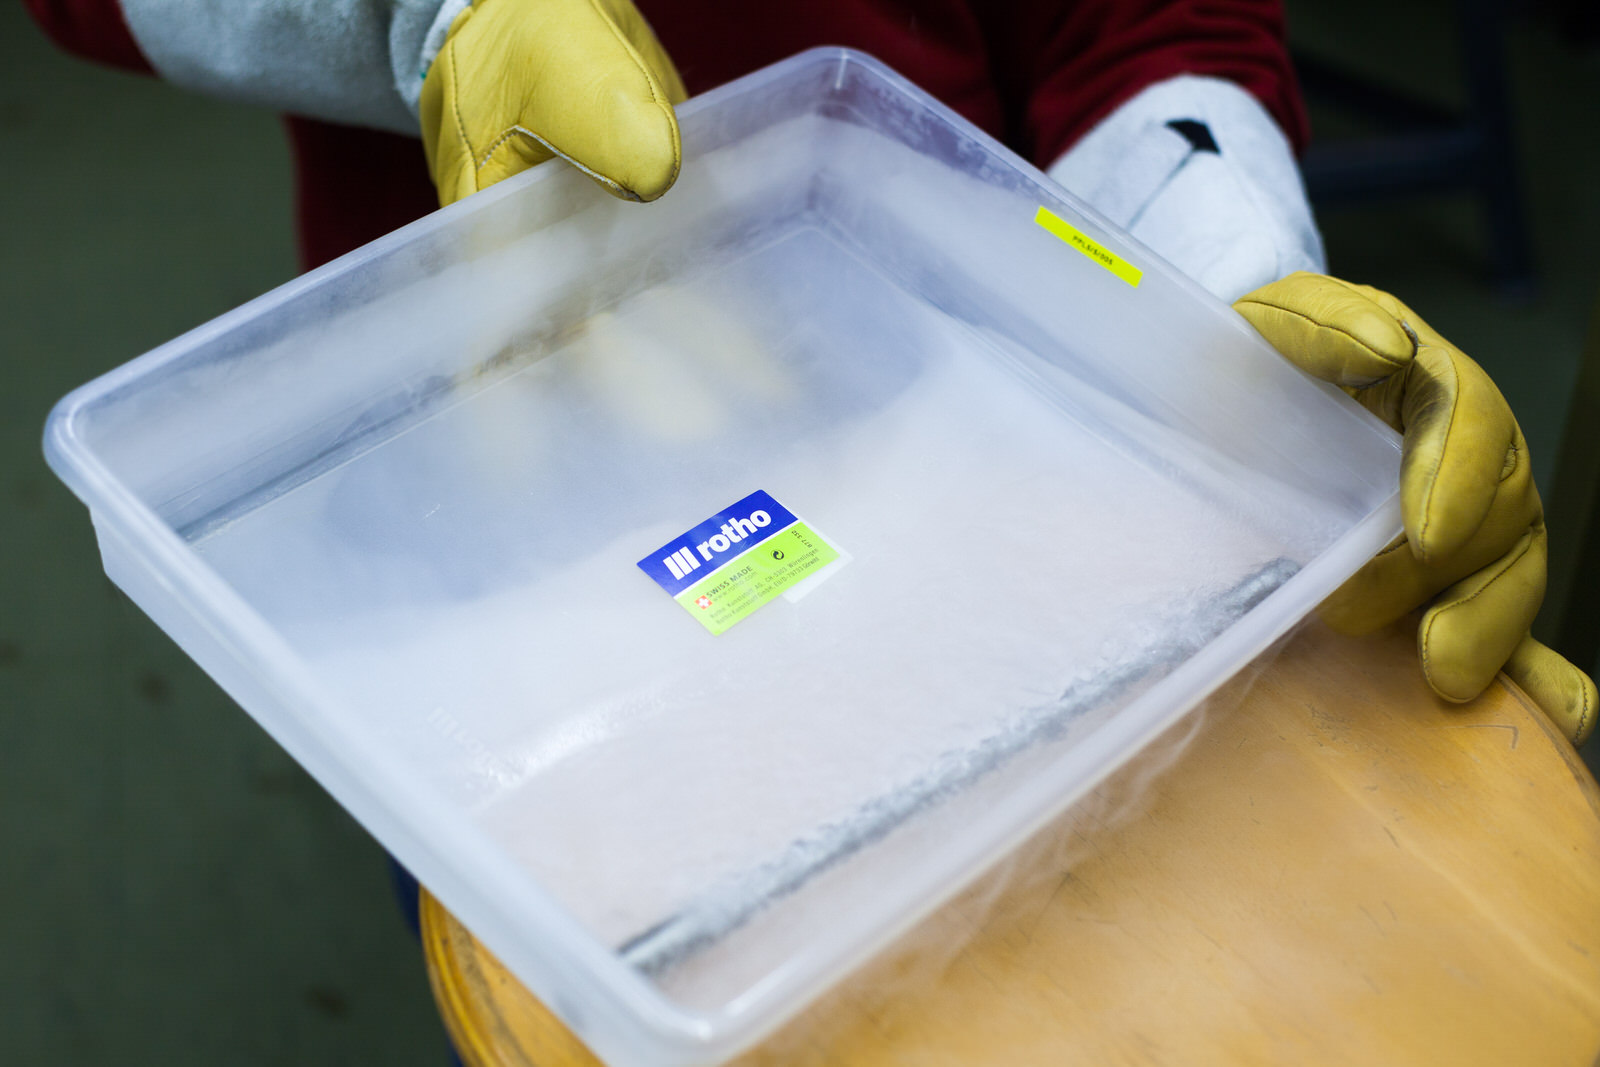
\includegraphics[width=\textwidth]{images/2/interferrometer-1}
\end{frame}

\begin{frame}
	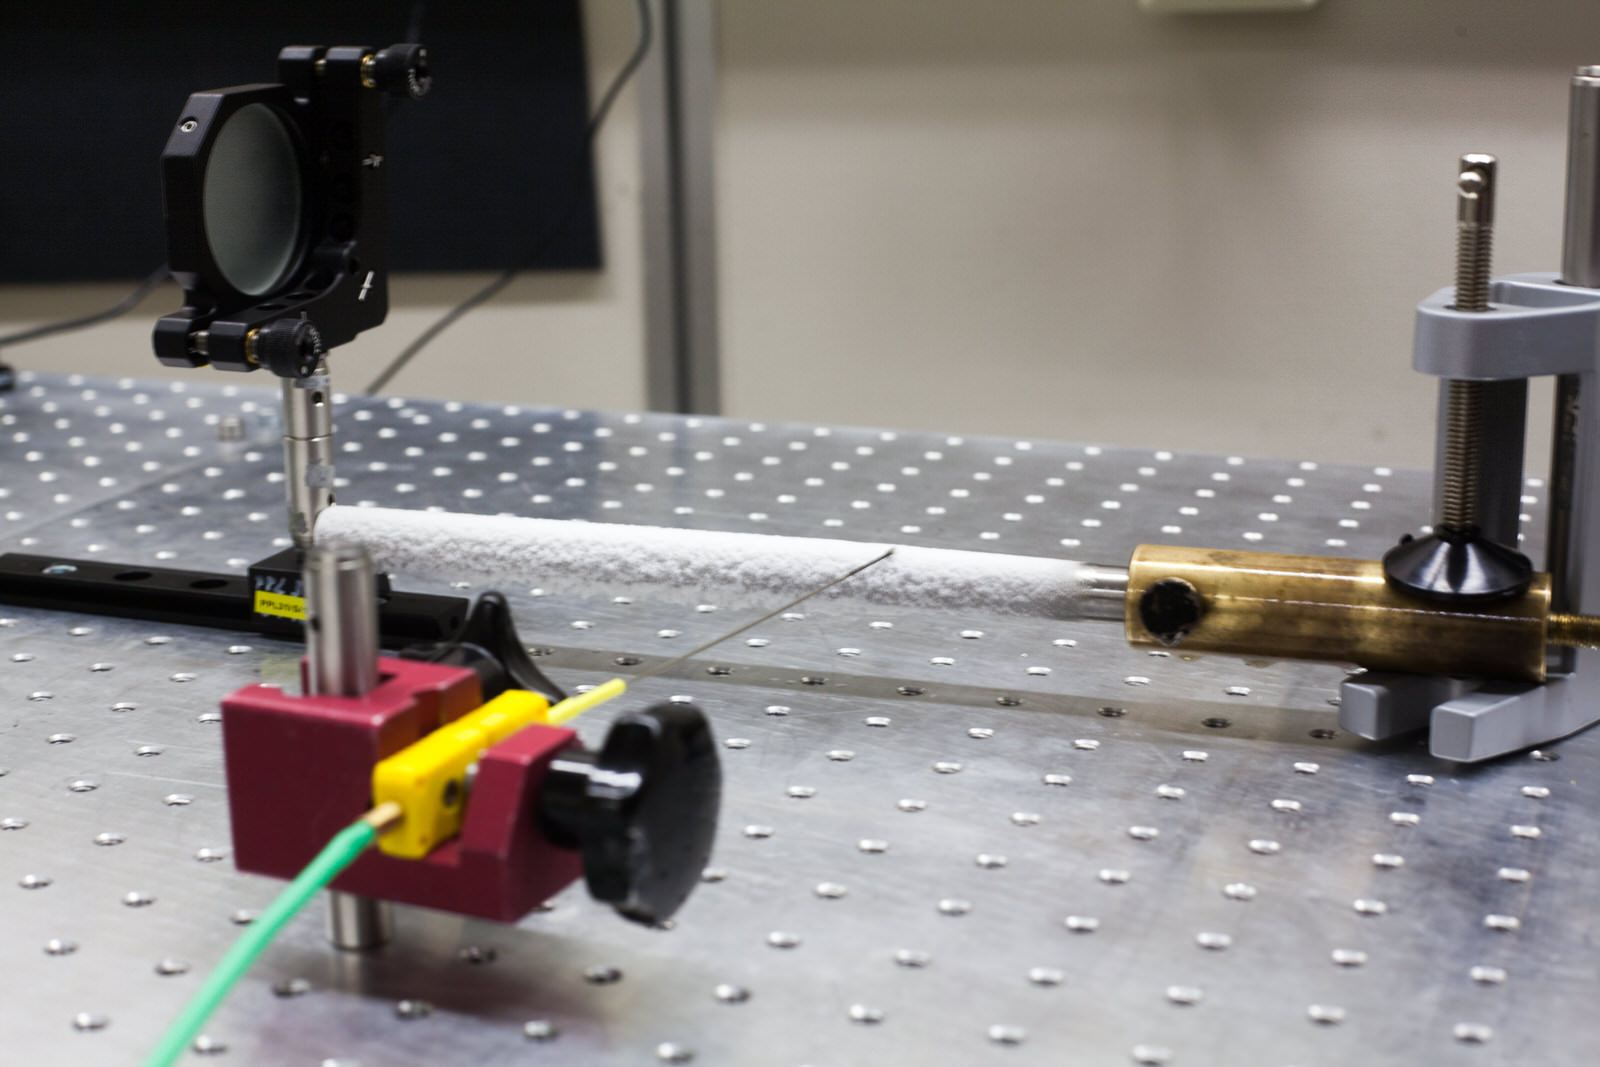
\includegraphics[width=\textwidth]{images/2/interferrometer-2}
\end{frame}

\begin{frame}
	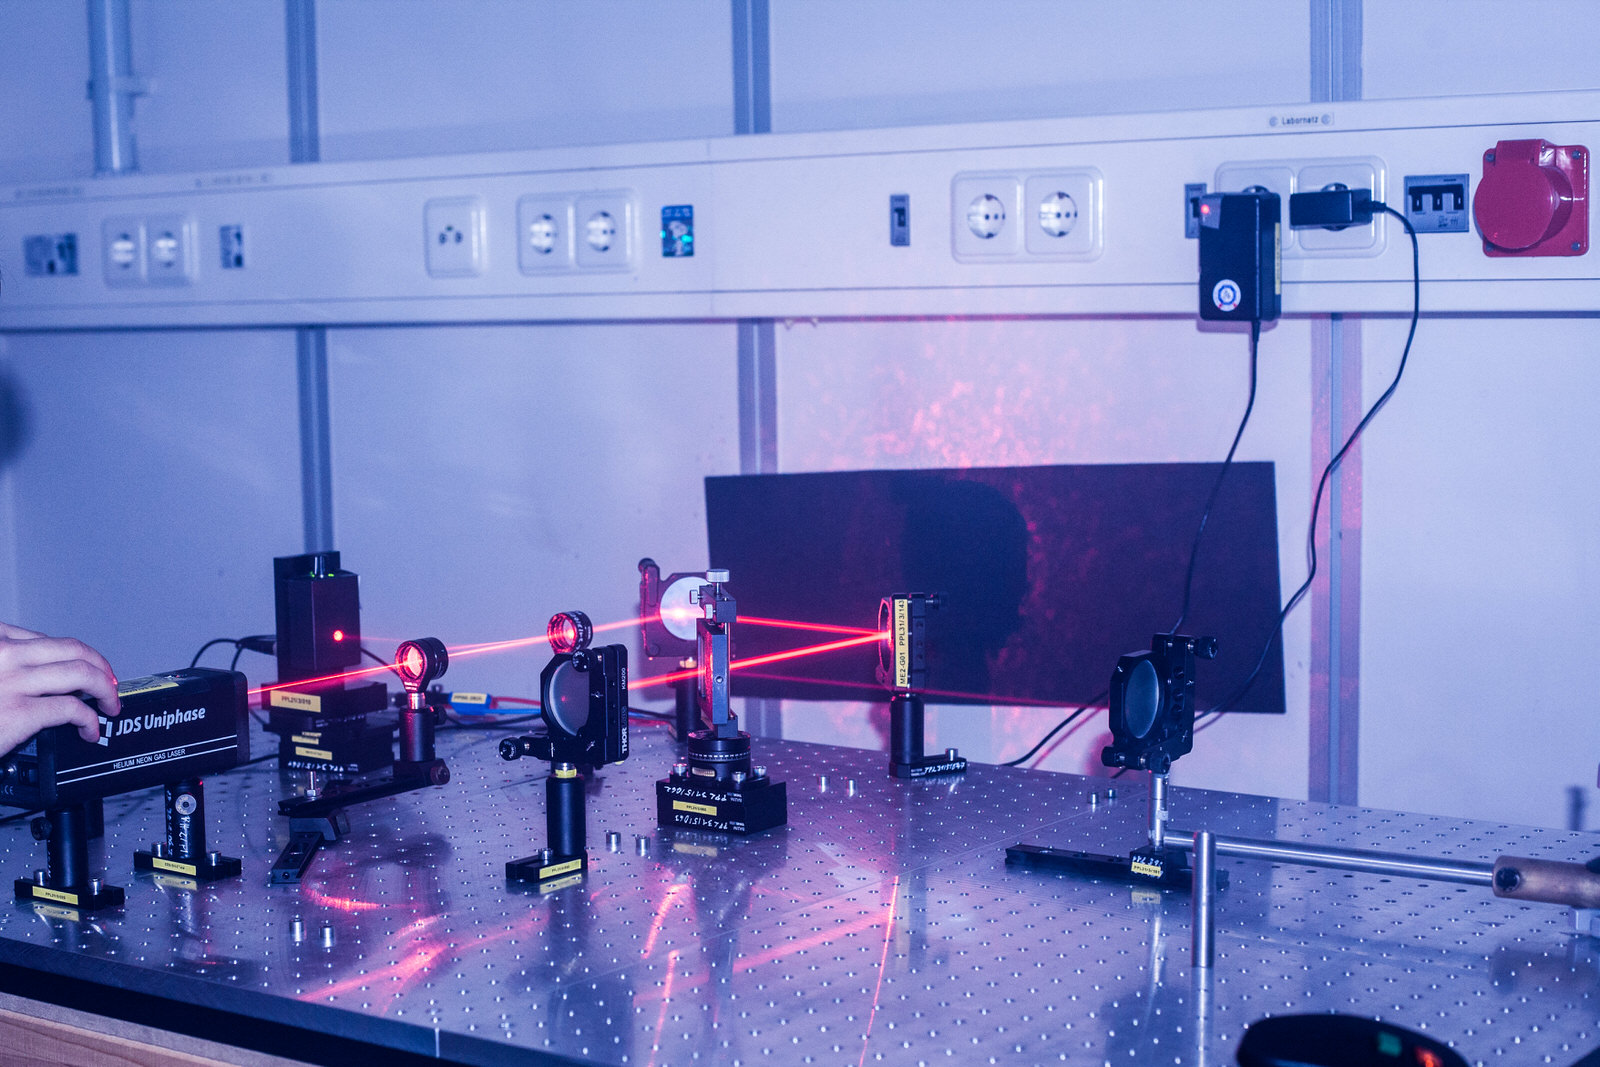
\includegraphics[width=\textwidth]{images/2/interferrometer-6}
\end{frame}


\section{Pitot}
\begin{frame}
	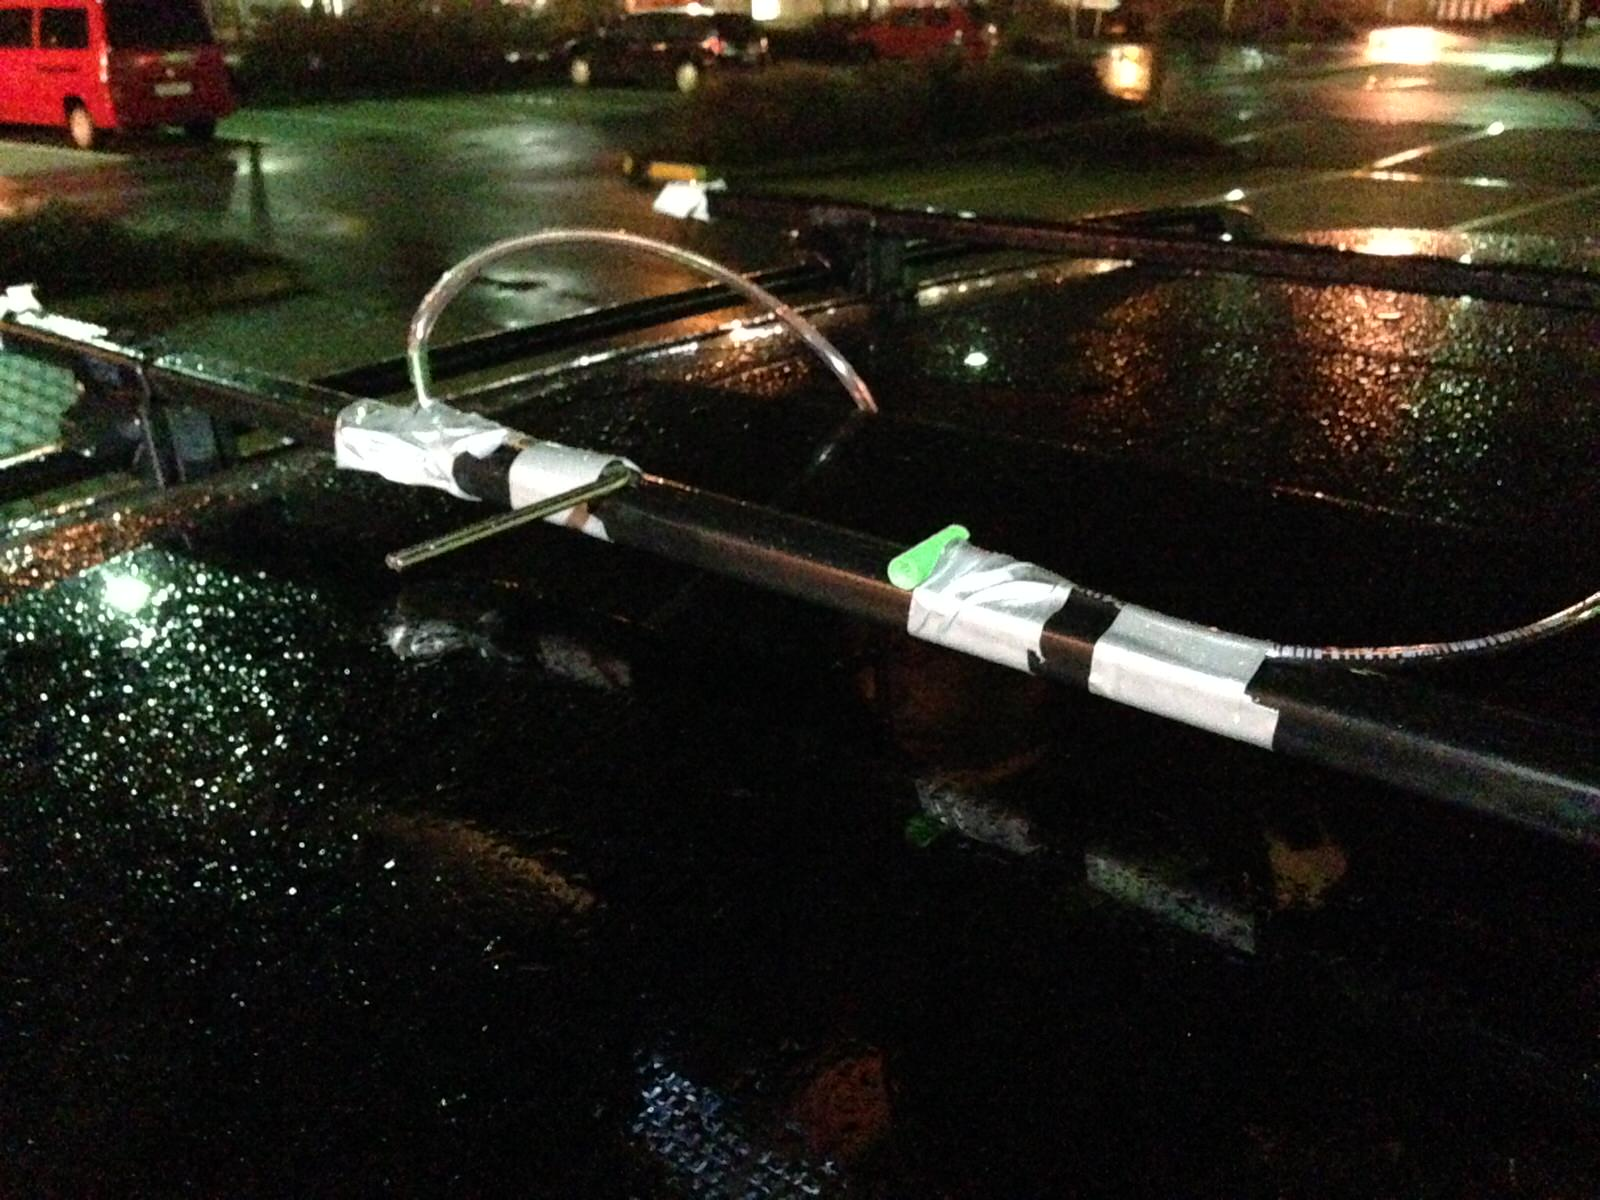
\includegraphics[width=\textwidth]{images/3/IMG_0004}
\end{frame}

\begin{frame}
	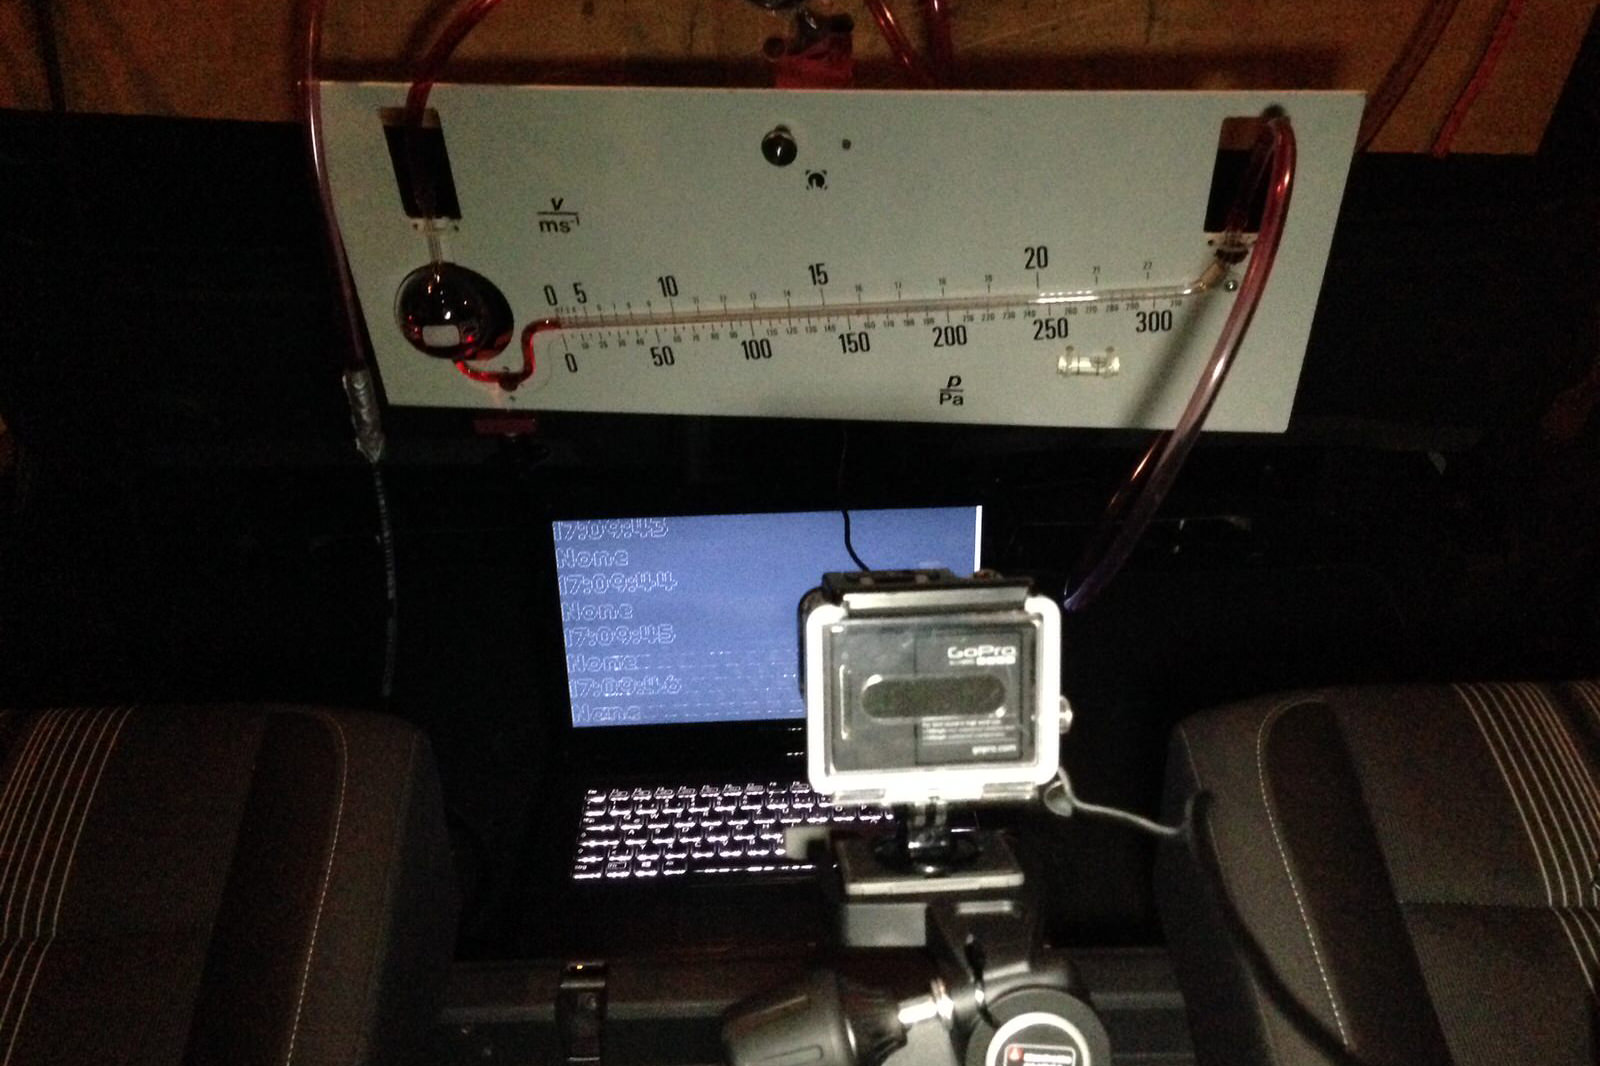
\includegraphics[width=\textwidth]{images/3/IMG_0007}
\end{frame}

\begin{frame}
	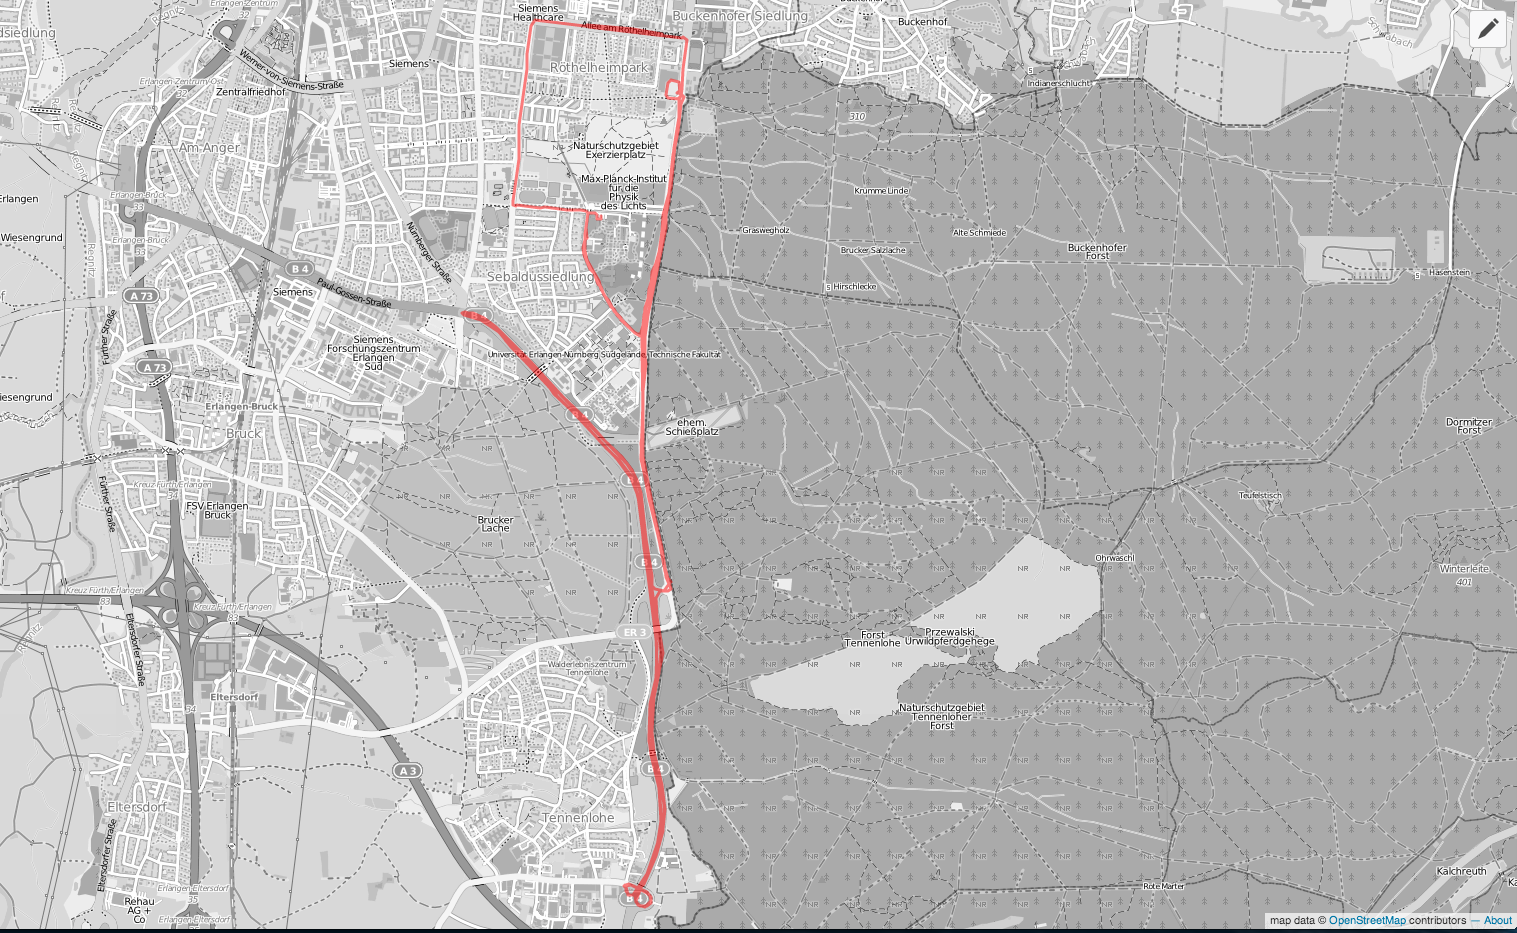
\includegraphics[width=\textwidth]{images/3/karte.png}
\end{frame}

\section{Doppelpendel}
\begin{frame}
\movie[showcontrols=false, autostart]{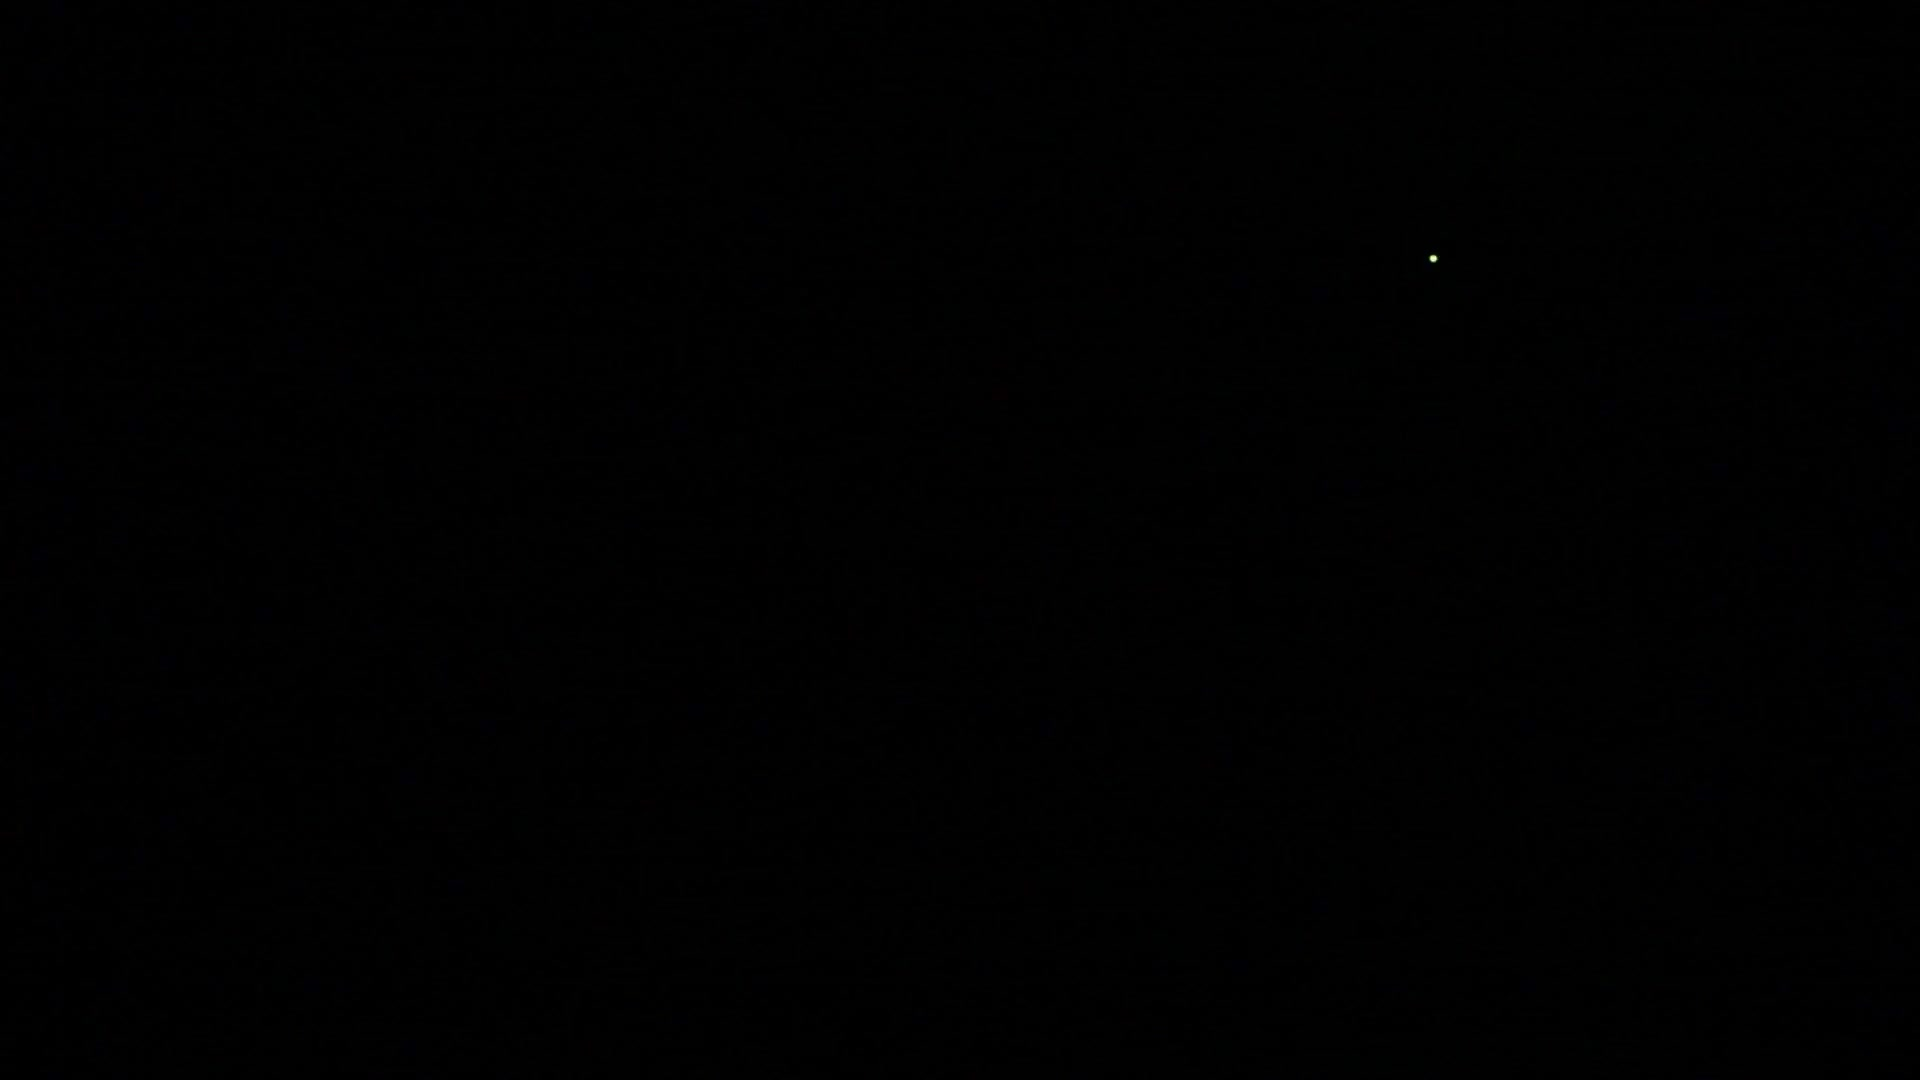
\includegraphics[width=\textwidth]{movies/6006_1}}{movies/6006.mov}
\end{frame}

\end{document}